

\section{Sentences and Annotations}\fbeg{}\begin{frame}{\ft{Viewing Sentence and Annotation Boundaries}}


\hspace*{-32pt}\begin{tikzpicture}

\node[anchor=south west,inner sep=0] (image) at (0,0){%

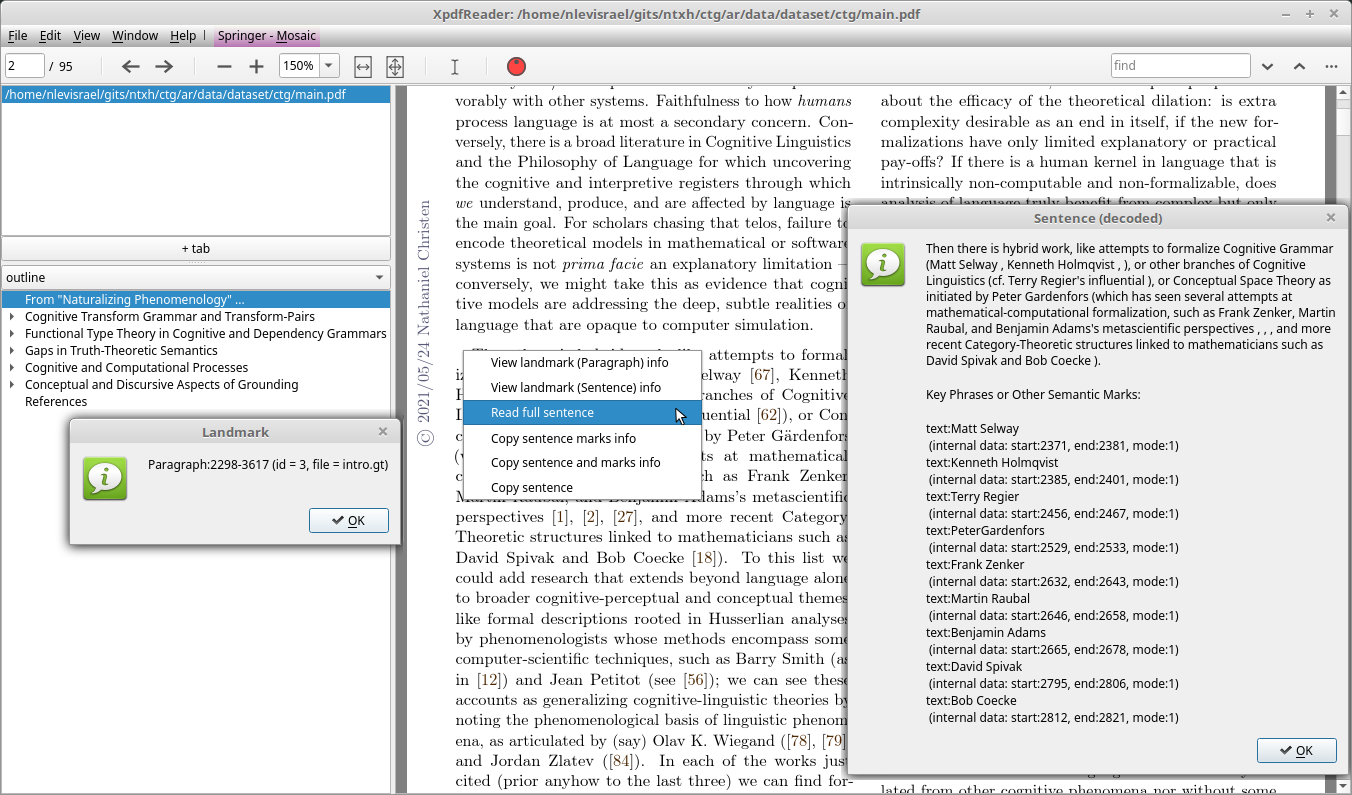
\includegraphics[scale=.595, clip, trim={138pt 0pt 76pt 23pt}]{ss/fin/ling.png}

};

\node[anchor=south west,inner sep=0] (image) at (13.2,0){%

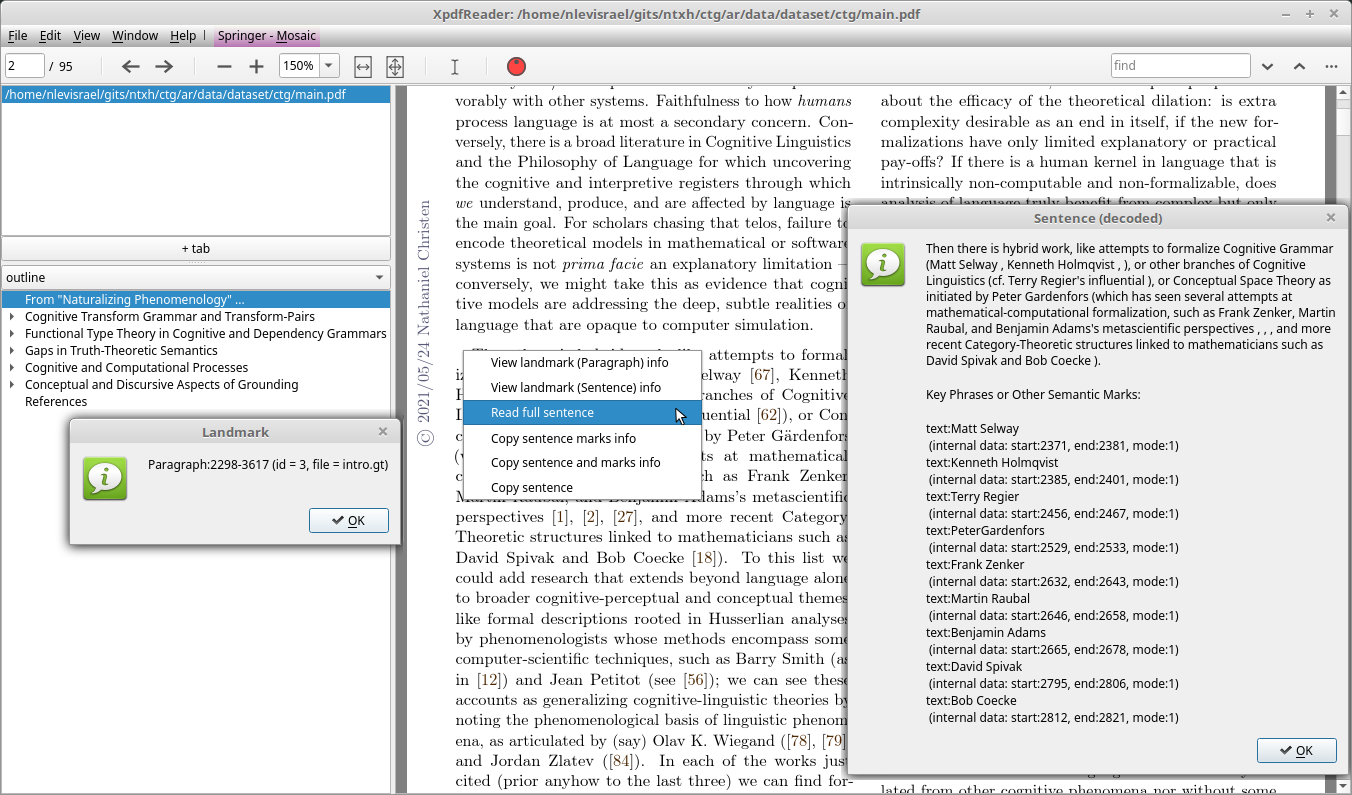
\includegraphics[scale=.595, clip, trim={843pt 0pt 2pt 23pt}]{ss/fin/ling.png}

};


\colorlet{bgbl}{green!63!blue}
\colorlet{bgblk}{bgbl!13!black}

\node [anchor=west,fill=bgblk!13,inner sep=12, 
opacity=0.88, text opacity=1] (note) at (2,3.4) {\hc{\hspace{2pt}\parbox{11cm}%
{Examining sentence\\contents and annotations}}};

\end{tikzpicture}


\end{frame}


